\documentclass[12pt, a4paper, dutch]{article}

% tikz is ugly, i don't bother making clean LaTeX code

\usepackage[margin=1in]{geometry}
\usepackage{circuitikz}
\usepackage{float}
\usepackage{babel}
\usepackage{siunitx}
\usepackage{amsmath}
\usepackage{scalerel}
\usepackage{csquotes}
\usepackage{parskip}
\usepackage{unicode-math}
\usepackage{fontspec}
\usepackage{tabularx}
\usepackage{booktabs}
\usepackage{graphicx}
\usepackage{pgfplots}
\usepackage{color}
\usepackage{hyperref}

\setmainfont{TeX Gyre Schola}
\setmathfont{TeX Gyre Schola Math}
\setmonofont{JetBrainsMono Nerd Font}
\sisetup{
	group-separator = {.},
	output-decimal-marker = {,}
}

\pgfplotsset{compat=newest}

\usetikzlibrary{calc}
\usetikzlibrary{shapes.geometric}
\usetikzlibrary{arrows.meta,arrows}
\usetikzlibrary{positioning}
\tikzset{
	initial/.style={circle, fill},
	final/.style={solid, double=white, circle, fill, thick, draw},
	decision/.style={diamond, black, draw},
	action/.style={rectangle, draw, rounded corners, align=center},
	arrow/.style={draw, -{Latex[length=3mm]}, thick, rounded corners}
}

\bigskipamount=7mm
\medskipamount=4mm
\parindent=0mm

\begin{document}

\begin{center}
\textbf{Ontwerp} \hspace{2mm} project Simon \hfill \textbf{Loek Le Blansch} (2180996)
\\\smallskip
\today
\end{center}

\medskip

Dit document maakt gebruik van hyperlinks, dus je kunt klikken op de blokken met
\emph{benadrukte tekst} om naar de definitie van dat blok te gaan.

\section{Software ontwerp}

\subsection*{Overzicht}\label{overzicht}
\begin{center}
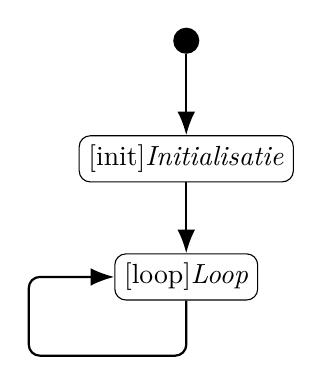
\begin{tikzpicture}[node distance=1.5cm]
\node[initial] (initial) at (0,0) {};
\node[action, below of = initial] (setup) {\hyperref[init]{\emph{Initialisatie}}};
\node[action, below of = setup] (loop) {\hyperref[loop]{\emph{Loop}}};

\draw [arrow] (initial) -- (setup);
\draw [arrow] (setup) -- (loop);
\draw [arrow] (loop) -- ++(0, -1) -- ++(-2, 0) -- ++(0, 1) -- (loop);

\end{tikzpicture}
\end{center}


\subsection*{Initialisatie}\label{init}
\begin{center}
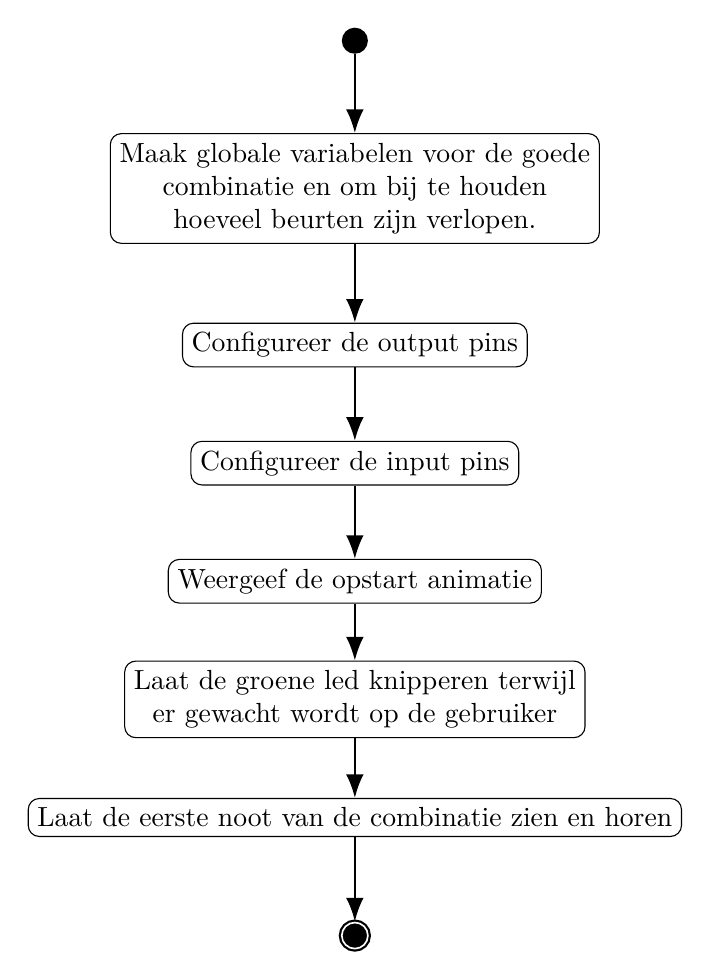
\begin{tikzpicture}[node distance=1.5cm]
\node[initial] (initial) at (0,0) {};

\node[action, below = 1cm of initial] (mkvars) {Maak globale variabelen voor de
	goede\\combinatie en om bij te houden\\hoeveel beurten zijn verlopen.};

\node[action, below = 1cm of mkvars] (outputs) {Configureer de output pins};
\node[action, below of = outputs] (inputs) {Configureer de input pins};


\node[action, below of = inputs] (bootanimation) {Weergeef de opstart animatie};

\node[action, below of = bootanimation] (waitready) {Laat de groene led knipperen
	terwijl\\er gewacht wordt op de gebruiker};

\node[action, below of = waitready] (simonsays) {Laat de eerste noot van de
	combinatie zien en horen};

\node[final, below of = simonsays] (final) {};

\draw [arrow] (initial) -- (mkvars);
\draw [arrow] (mkvars) -- (outputs);
\draw [arrow] (outputs) -- (inputs);
\draw [arrow] (inputs) -- (bootanimation);
\draw [arrow] (bootanimation) -- (waitready);
\draw [arrow] (waitready) -- (simonsays);
\draw [arrow] (simonsays) -- (final);

\end{tikzpicture}
\end{center}


\subsection*{Loop}\label{loop}
\begin{center}
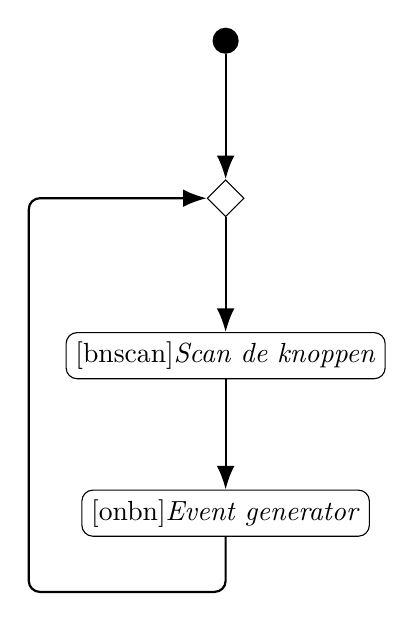
\begin{tikzpicture}[node distance=2cm]
\node[initial] (initial) at (0,0) {};

\node[decision, below of = initial] (begin) {};

\node[action, below of = begin] (scanbn)
	{\hyperref[bnscan]{\emph{Scan de knoppen}}};
\node[action, below of = scanbn] (bngenerator)
	{\hyperref[onbn]{\emph{Event generator}}};

\draw [arrow] (initial) -- (begin);
\draw [arrow] (begin) -- (scanbn);
\draw [arrow] (scanbn) -- (bngenerator);

\draw [arrow] (bngenerator) -- ++(0, -1) -- ++(-2.5, 0) |- (begin);

\end{tikzpicture}
\end{center}


\subsection*{Knoppen scan}\label{bnscan}
\begin{center}
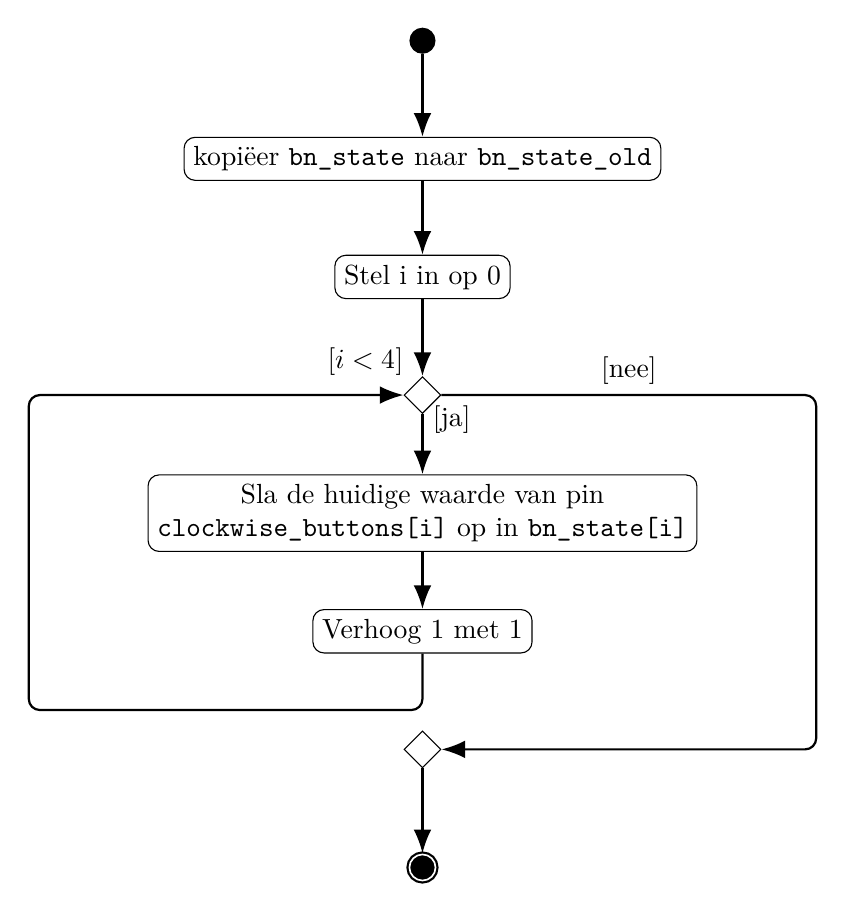
\begin{tikzpicture}[node distance=1.5cm]

\node[initial] (initial) at (0,0) {};

\node[action, below of = initial] (mvarr)
	{kopi\"eer \texttt{bn\_state} naar \texttt{bn\_state\_old}};

\node[action, below of = mvarr] (ie0) {Stel i in op 0};
\node[decision, below of = ie0,
	label={above left:[$i<4$]}] (iloopstart) {};

\node[action, below of = iloopstart] (checkpin)
	{Sla de huidige waarde van pin\\\texttt{clockwise\_buttons[i]} op in
	\texttt{bn\_state[i]}};

\node[action, below of = checkpin] (ip1)
	{Verhoog 1 met 1};

\node[decision, below of = ip1] (iloopend) {};

\node[final, below of = iloopend] (final) {};


\draw [arrow] (initial) -- (mvarr);
\draw [arrow] (mvarr) -- (ie0);
\draw [arrow] (checkpin) -- (ip1);
\draw [arrow] (iloopend) -- (final);

\draw [arrow] (iloopstart) node[below right]{[ja]} -- (checkpin);

\draw [arrow] (ie0) -- (iloopstart);

\draw [arrow] (iloopstart) -- node[above]{[nee]} ++(5.0, 0) |- (iloopend);

\draw [arrow] (ip1) -- ++(0, -1) -- ++(-5.0, 0) |- (iloopstart);

\end{tikzpicture}
\end{center}


\subsection*{Event generator}\label{onbn}
\begin{center}
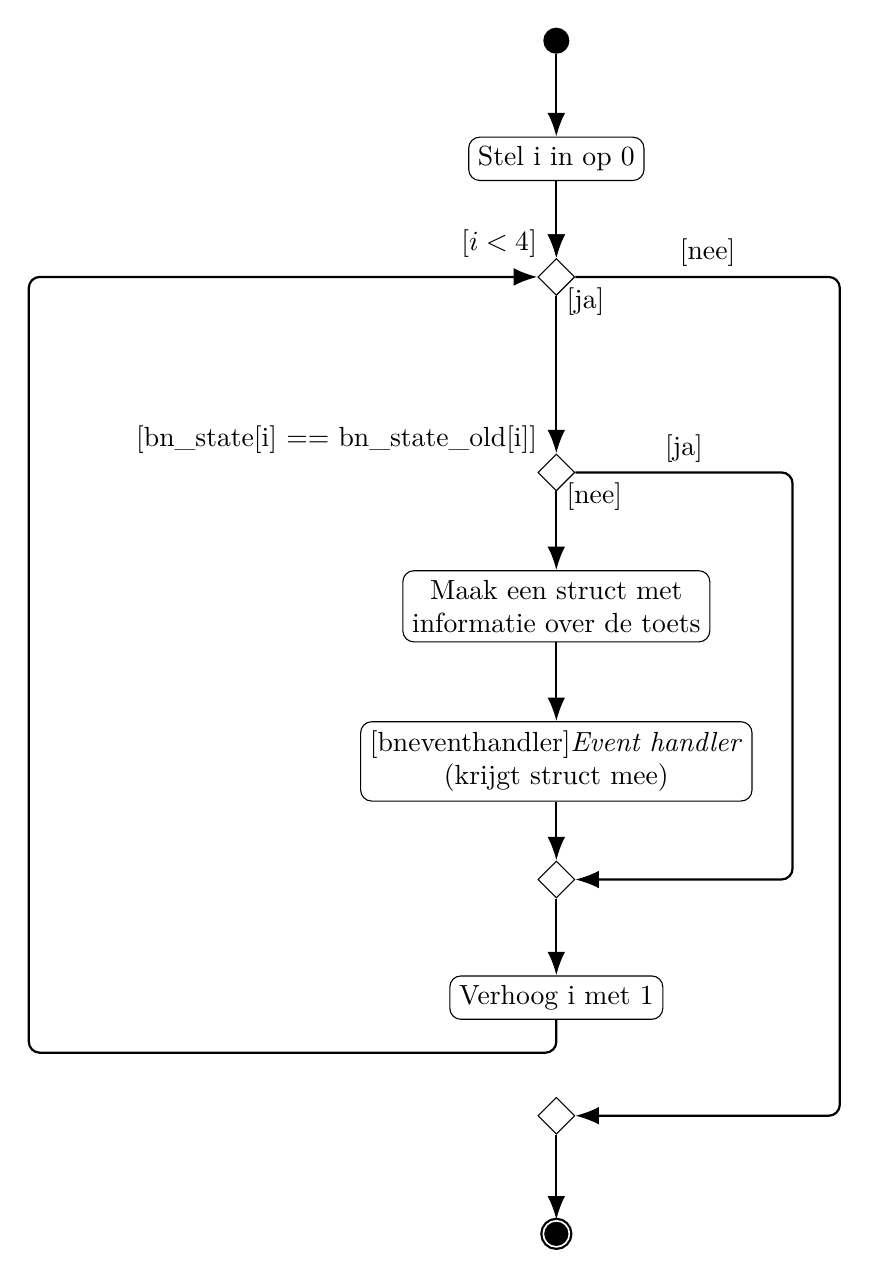
\begin{tikzpicture}[node distance=1.5cm]
\node[initial] (initial) at (0,0) {};

\node[action, below of = initial] (ie0) {Stel i in op 0};
\node[decision, below of = ie0,
	label={above left:[$i < 4$]}] (iloopstart) {};
\node[decision, below = 2cm of iloopstart,
	label={above left:[bn\_state[i] == bn\_state\_old[i]]}] (bndiff) {};
\node[action, below = 1cm of bndiff] (makestruct)
	{Maak een struct met\\informatie over de toets};
\node[action, below = 1cm of makestruct] (bnhandl)
	{\hyperref[bneventhandler]{\emph{Event handler}}\\(krijgt struct mee)};
\node[decision, below of = bnhandl] (merge) {};
\node[action, below of = merge] (ip1)
	{Verhoog i met 1};
\node[decision, below of = ip1] (iloopend) {};

\node[final, below of = iloopend] (final) {};

\draw [arrow] (initial) -- (ie0);
\draw [arrow] (ie0) -- (iloopstart);

\draw [arrow] (ip1) -- ++(0, -0.7) -- ++(-6.7, 0) |- (iloopstart);
\draw [arrow] (ie0) -- (iloopstart);
\draw [arrow] (iloopstart) node[below right]{[ja]} -- (bndiff);
\draw [arrow] (iloopstart) -- node[above]{[nee]} ++(3.6, 0) |- (iloopend);

\draw [arrow] (bndiff) -- node[above]{[ja]} ++(3, 0) |- (merge);
\draw [arrow] (bndiff) node[below right]{[nee]} -- (makestruct);

\draw [arrow] (makestruct) -- (bnhandl);
\draw [arrow] (bnhandl) -- (merge);
\draw [arrow] (merge) -- (ip1);
\draw [arrow] (iloopend) -- (final);

\end{tikzpicture}
\end{center}


\subsection*{Event handler}\label{bneventhandler}
\begin{center}
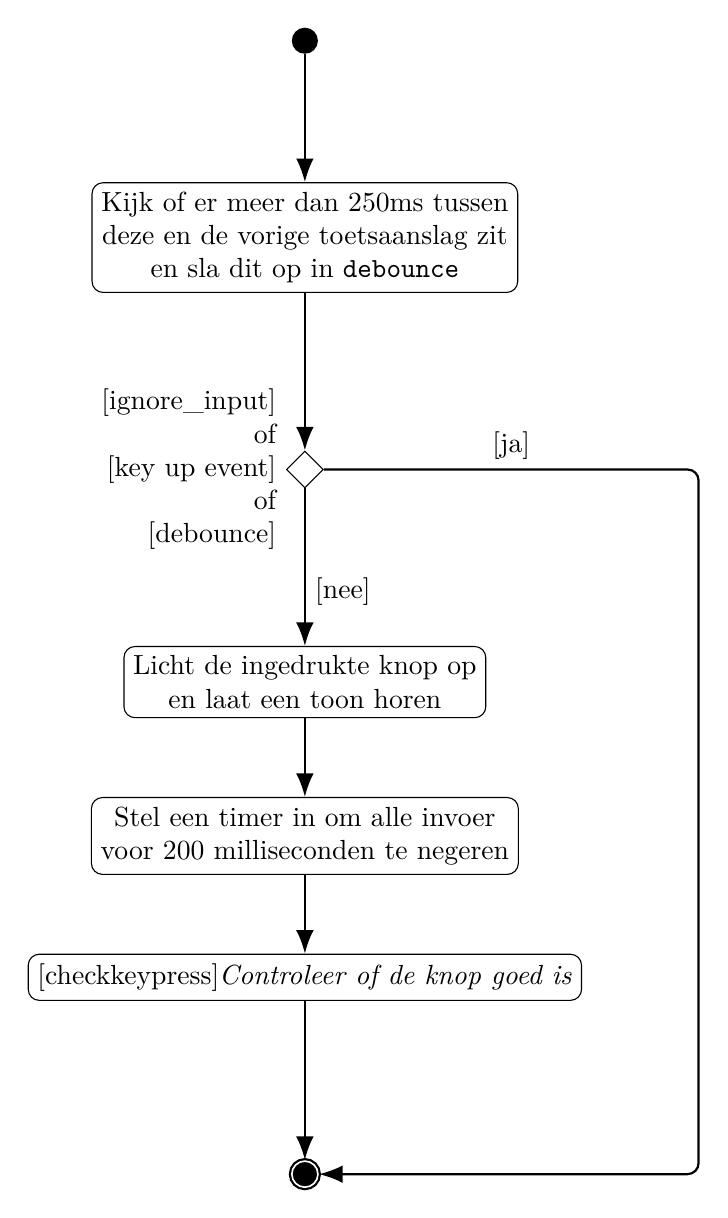
\begin{tikzpicture}[node distance=2.5cm]

\node[initial] (initial) at (0,0) {};

\node[action, below of = initial] (debounce)
	{Kijk of er meer dan 250ms tussen\\deze en de vorige toetsaanslag zit\\en sla dit
	op in \texttt{debounce}};

\node [decision, below = 2cm of debounce,
	label={[align=right]left:{[ignore\_input]\\of\\{}[key up
	event]\\of\\{}[debounce]}}] (fastreturn) {};

\node[action, below = 2cm of fastreturn] (av)
	{Licht de ingedrukte knop op\\en laat een toon horen};

\node[action, below = 1cm of av] (ignoreinput)
	{Stel een timer in om alle invoer\\voor 200 milliseconden te negeren};

\node[action, below = 1cm of ignoreinput] (checkkp)
	{\hyperref[checkkeypress]{\emph{Controleer of de knop goed is}}};

\node[final, below of = checkkp] (final) {};

\draw [arrow] (initial) -- (debounce);
\draw [arrow] (debounce) -- (fastreturn);
\draw [arrow] (fastreturn) -- node[midway,above]{[ja]} ++(5, 0) |- (final);
\draw [arrow] (fastreturn) -- node[below right]{[nee]} (av);
\draw [arrow] (av) -- (ignoreinput);
\draw [arrow] (ignoreinput) -- (checkkp);
\draw [arrow] (checkkp) -- (final);

\end{tikzpicture}
\end{center}


\subsection*{Controleer of de knop goed is}\label{checkkeypress}
\begin{center}
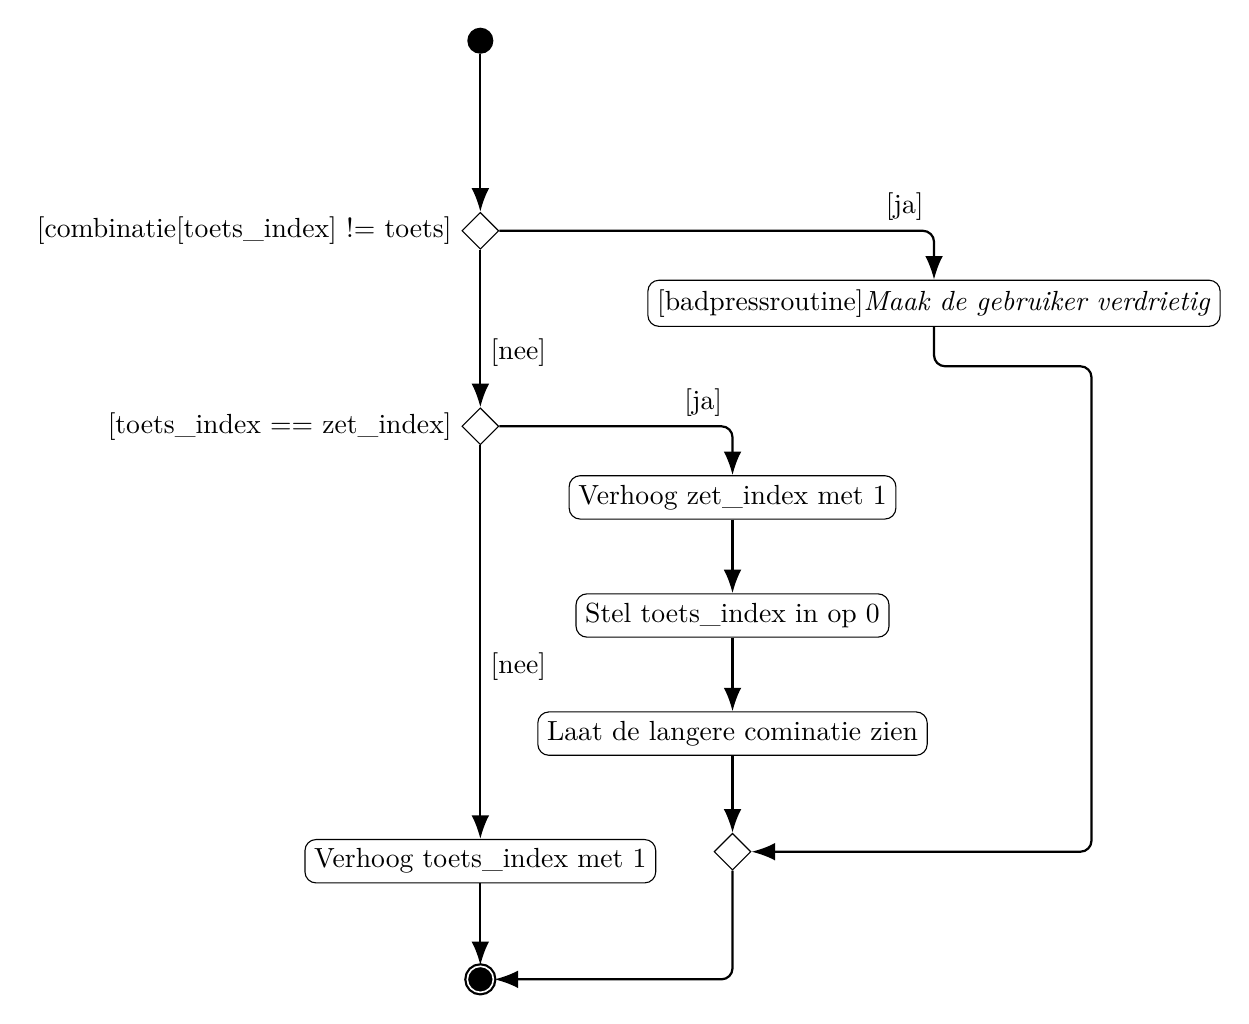
\begin{tikzpicture}[node distance=1.5cm]

\node[initial] (initial) at (0,0) {};

\node [decision, below = 2cm of initial,
	label={left:{[combinatie[toets\_index] != toets]}}] (fastreturn1) {};

\node[action, below right = 5mm and 2cm of fastreturn1] (badpressroutine)
	{\hyperref[badpressroutine]{\emph{Maak de gebruiker verdrietig}}};

\node [decision, below = 2cm of fastreturn1,
	label={left:{[toets\_index == zet\_index]}}] (fastreturn2) {};

\node[action, below right = 5mm and 1cm of fastreturn2] (turnnumberpp)
	{Verhoog zet\_index met 1};

\node[action, below of = turnnumberpp] (ennume0)
	{Stel toets\_index in op 0};

\node[action, below of = ennume0] (newcomb)
	{Laat de langere cominatie zien};

\node [decision, below of = newcomb] (comb1) {};

\node[action, below = 5cm of fastreturn2] (ennumpp)
	{Verhoog toets\_index met 1};

\node[final, below of = ennumpp] (final) {};

\draw [arrow] (initial) -- (fastreturn1);
\draw [arrow] (fastreturn1) -| node[above left]{[ja]} (badpressroutine);
\draw [arrow] (fastreturn2) -| node[above left]{[ja]} (turnnumberpp);
\draw [arrow] (turnnumberpp) -- (ennume0);
\draw [arrow] (ennume0) -- (newcomb);
\draw [arrow] (newcomb) -- (comb1);
\draw [arrow] (fastreturn1) -- node[below right]{[nee]} (fastreturn2);
\draw [arrow] (fastreturn2) -- node[below right]{[nee]} (ennumpp);
\draw [arrow] (badpressroutine) |- ++(2, -0.8) |- (comb1);
\draw [arrow] (ennumpp) -- (final);
\draw [arrow] (comb1) |- (final);

\end{tikzpicture}
\end{center}


\subsection*{Verkeerde knop routine}\label{badpressroutine}
\begin{center}
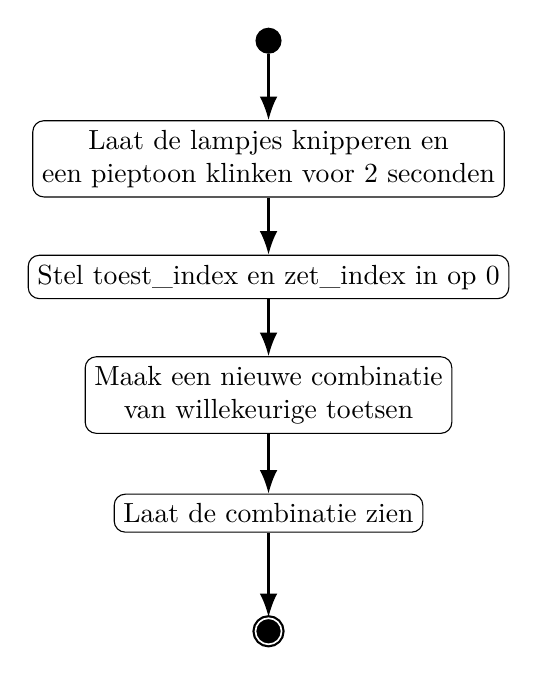
\begin{tikzpicture}[node distance=1.5cm]

\node[initial] (initial) at (0,0) {};

\node[action, below of = initial] (av)
	{Laat de lampjes knipperen en\\een pieptoon klinken voor 2 seconden};

\node[action, below of = av] (resetvars)
	{Stel toest\_index en zet\_index in op 0};

\node[action, below of = resetvars] (newcomb)
	{Maak een nieuwe combinatie\\van willekeurige toetsen};

\node[action, below of = newcomb] (showcomb)
	{Laat de combinatie zien};

\node[final, below of = showcomb] (final) {};

\draw [arrow] (initial) -- (av);
\draw [arrow] (av) -- (resetvars);
\draw [arrow] (resetvars) -- (newcomb);
\draw [arrow] (newcomb) -- (showcomb);
\draw [arrow] (showcomb) -- (final);

\end{tikzpicture}
\end{center}

\section{Hardware}

\subsection{Schema}

\begin{center}
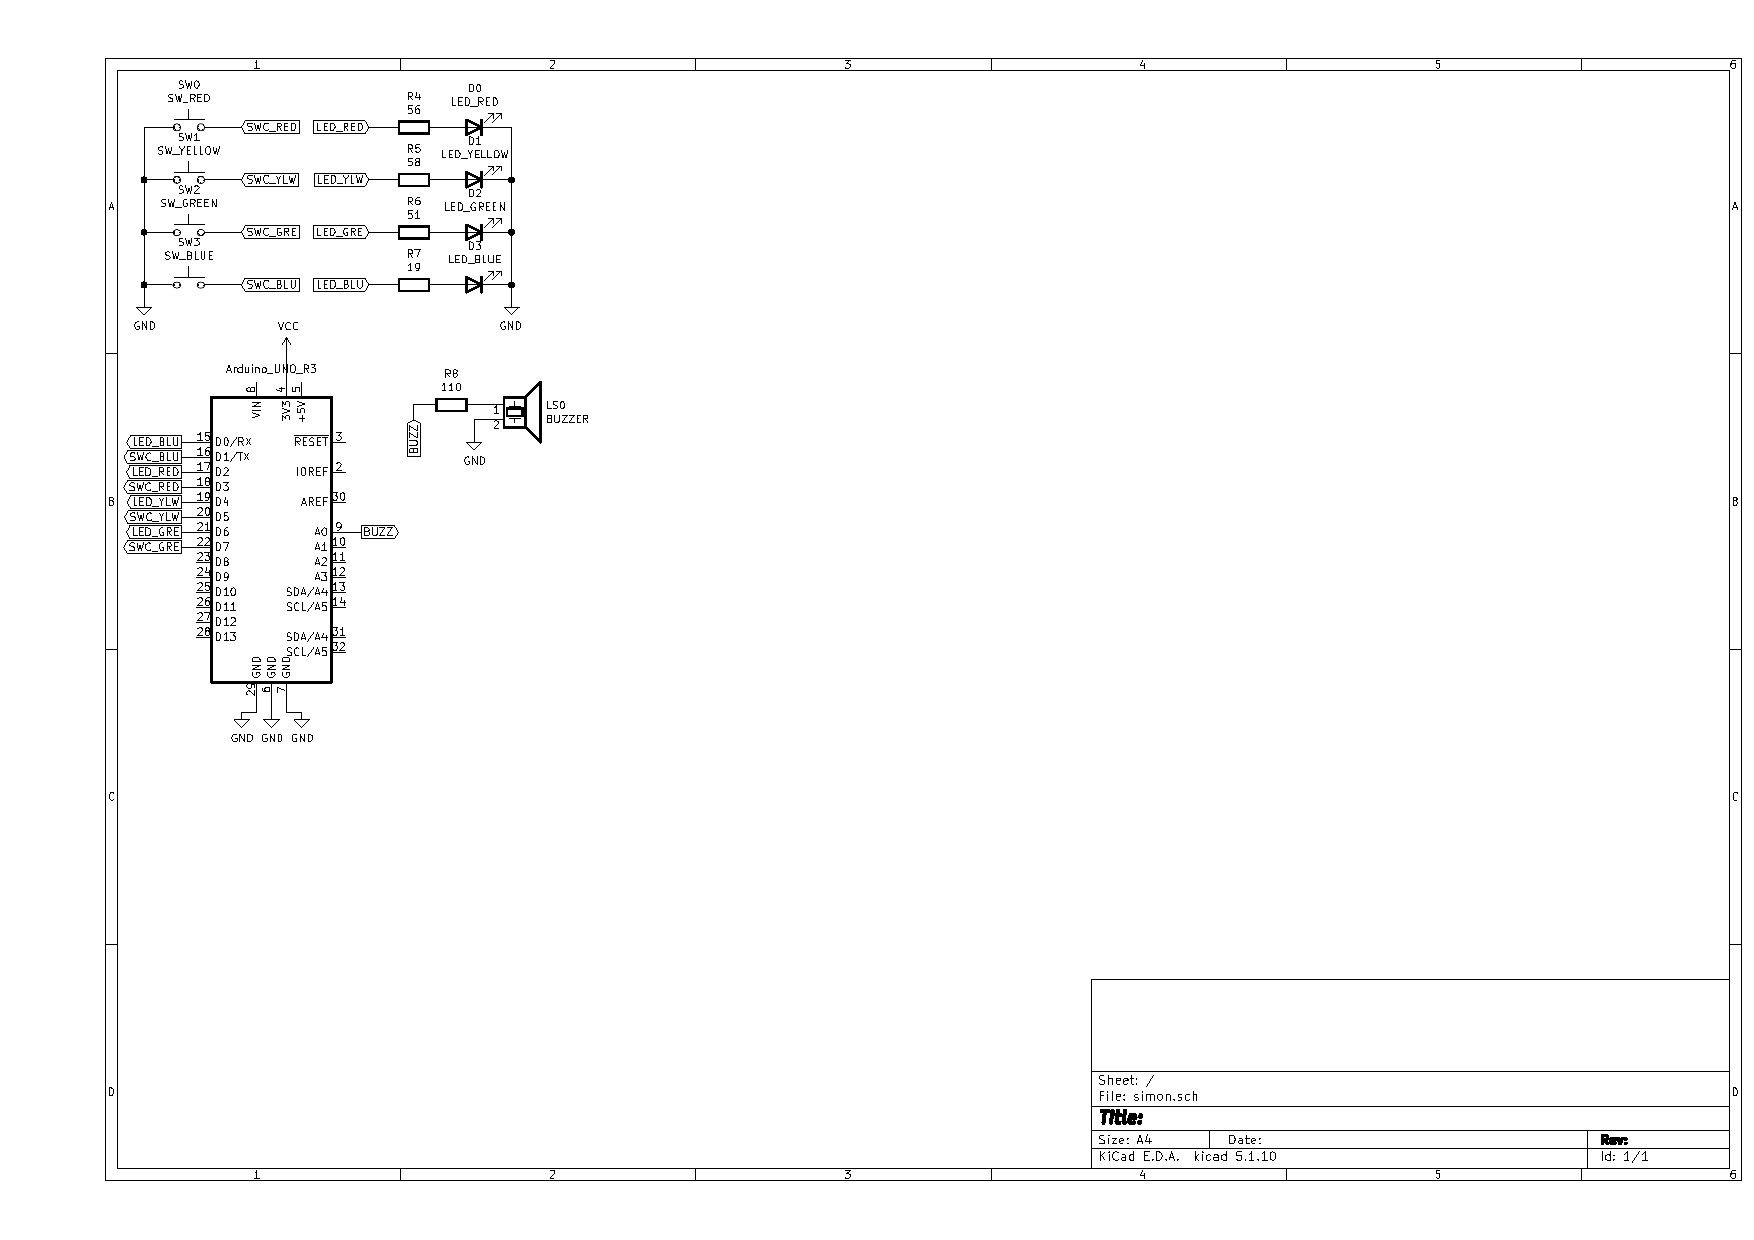
\includegraphics[
	clip,
	trim=21mm 83mm 197mm 13mm,
	width=9cm
]{./schema.pdf}
\end{center}

\subsection{PCB}
\begin{center}
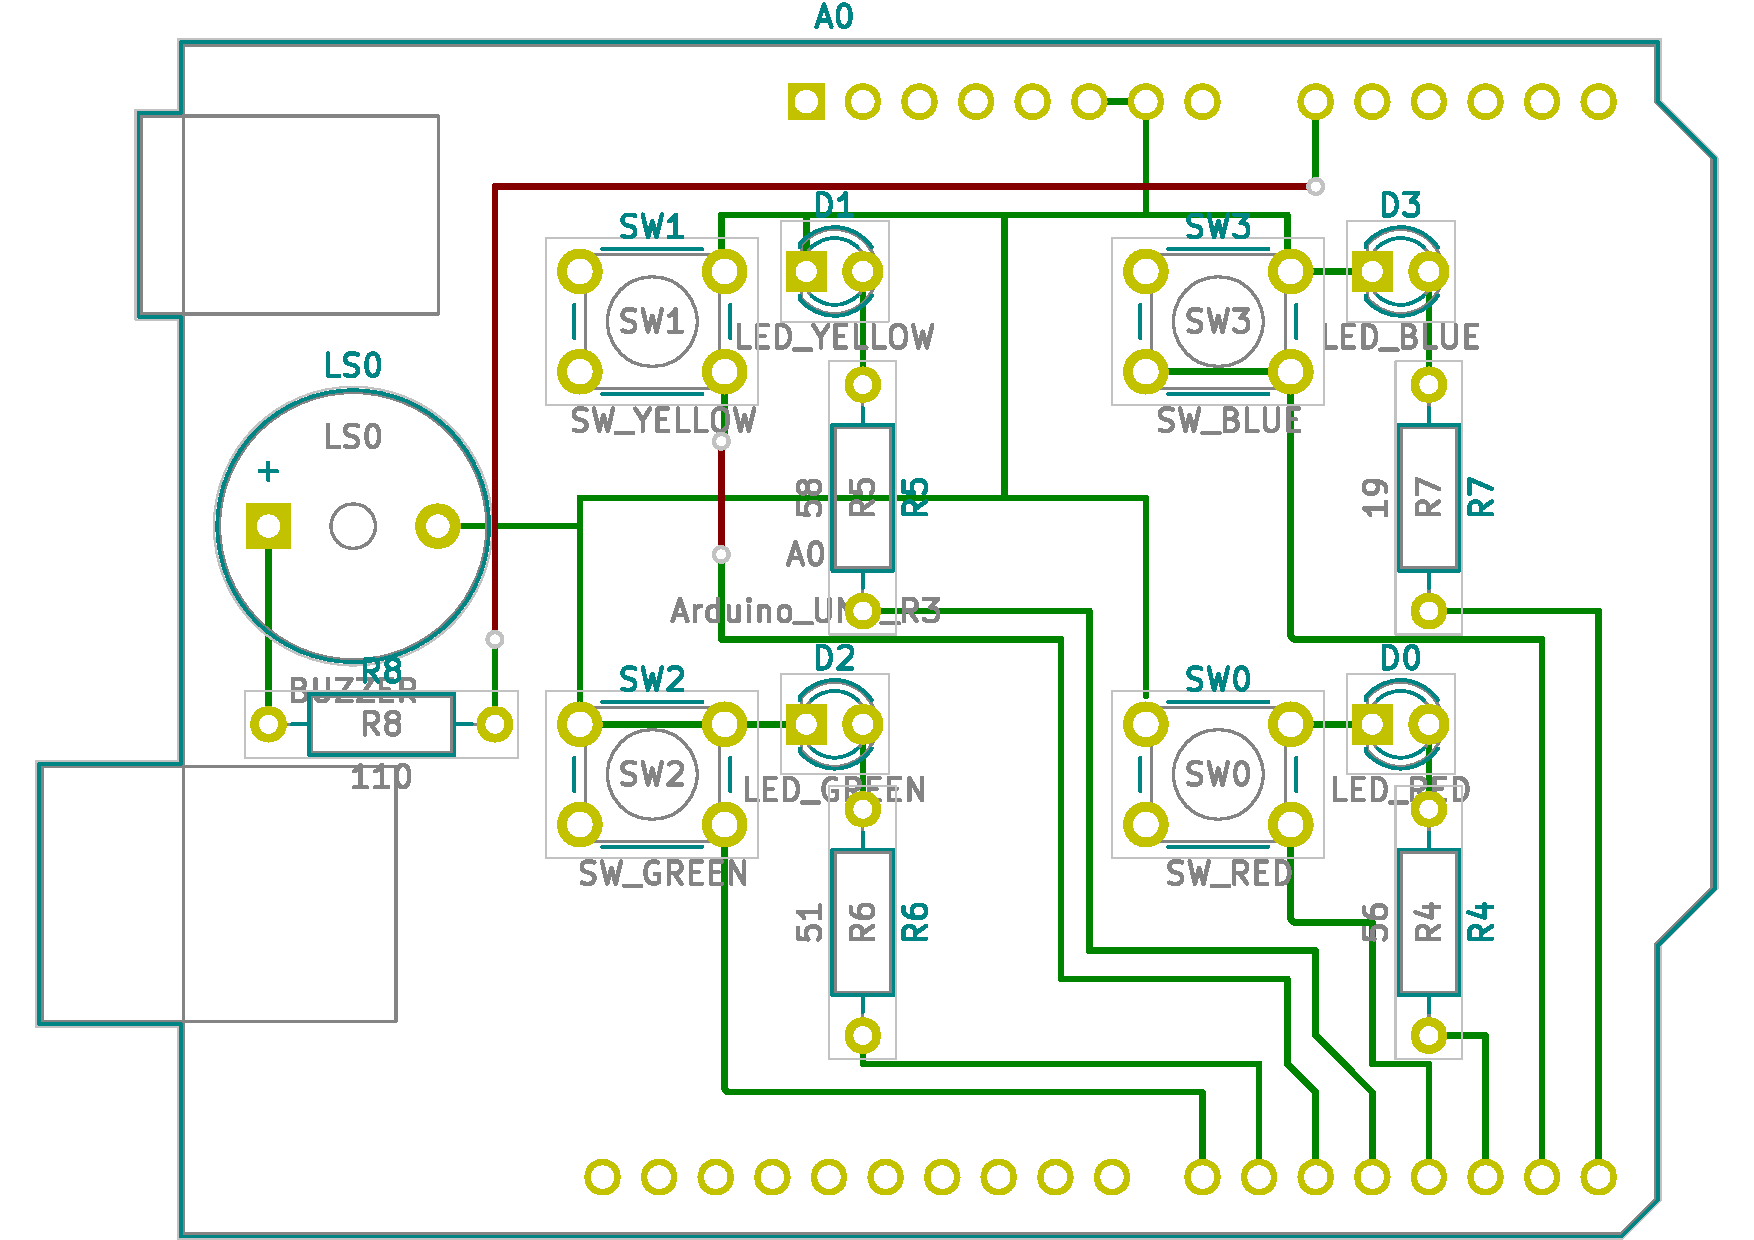
\includegraphics[
	width=9cm
]{./pcb.pdf}
\end{center}

\end{document}
